\documentclass{ximera}
%\usepackage{todonotes}

\usepackage{tkz-euclide}
\usetikzlibrary{backgrounds} %% for boxes around graphs
\usetikzlibrary{shapes,positioning}  %% Clouds and stars
\usetkzobj{all}
\usepackage[makeroom]{cancel} %% for strike outs
%\usepackage{mathtools} %% for pretty underbrace % Breaks Ximera
\usepackage{multicol}


\newcommand{\RR}{\mathbb R}
\renewcommand{\d}{\,d}
\newcommand{\dd}[2][]{\frac{d #1}{d #2}}
\renewcommand{\l}{\ell}
\newcommand{\ddx}{\frac{d}{dx}}
\newcommand{\zeroOverZero}{$\boldsymbol{\tfrac{0}{0}}$}
\newcommand{\numOverZero}{$\boldsymbol{\tfrac{\#}{0}}$}
\newcommand{\dfn}{\textbf}
\newcommand{\eval}[1]{\bigg[ #1 \bigg]}
\renewcommand{\epsilon}{\varepsilon}
\renewcommand{\iff}{\Leftrightarrow}

\DeclareMathOperator{\arccot}{arccot}
\DeclareMathOperator{\arcsec}{arcsec}
\DeclareMathOperator{\arccsc}{arccsc}


\colorlet{textColor}{black} 
\colorlet{background}{white}
\colorlet{penColor}{blue!50!black} % Color of a curve in a plot
\colorlet{penColor2}{red!50!black}% Color of a curve in a plot
\colorlet{penColor3}{red!50!blue} % Color of a curve in a plot
\colorlet{penColor4}{green!50!black} % Color of a curve in a plot
\colorlet{penColor5}{orange!80!black} % Color of a curve in a plot
                                      \colorlet{fill1}{blue!50!black!20} % Color of fill in a plot
\colorlet{fill2}{blue!10} % Color of fill in a plot
\colorlet{fillp}{fill1} % Color of positive area
\colorlet{filln}{red!50!black!20} % Color of negative area
\colorlet{gridColor}{gray!50} % Color of grid in a plot

\pgfmathdeclarefunction{gauss}{2}{% gives gaussian
  \pgfmathparse{1/(#2*sqrt(2*pi))*exp(-((x-#1)^2)/(2*#2^2))}%
}



\newcommand{\fullwidth}{}
\newcommand{\normalwidth}{}



%% makes a snazzy t-chart for evaluating functions
\newenvironment{tchart}{\rowcolors{2}{}{background!90!textColor}\array}{\endarray}

%%This is to help with formatting on future title pages.
\newenvironment{sectionOutcomes}{}{} 

\author{Emma Smith Zbarsky}
\license{Creative Commons Attribution 3.0 Unported}
\acknowledgement{https://quadbase.org/questions/q14357v1}
\begin{document}

\begin{exercise}

Calculate $\frac{df}{dy}$ of \[f(y) = \sin\left(\arctan(3y)\right).\]


\begin{hint}
This problem involves derivatives of inverse trigonometric functions and
the use of trigonometric triangles for substitutions.
\end{hint}


\begin{hint}
\begin{align*}
f'(y) &= \frac{d}{dy}\left(\sin\left(\arctan(3y)\right)\right) \\
&= \cos(\arctan(3y))\frac{d}{dy}\left(\arctan(3y)\right) \\
&=  \frac{1}{\sqrt{1+9y^2}}\left(\frac{3}{1+9y^2}\right) \\
&= \frac{3}{\left(1+9y^2\right)^{3/2}}
\end{align*}

where we have used 

\begin{image}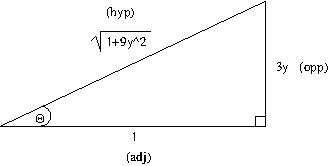
\includegraphics{trig-triangle-arctan3y.jpg}\end{image}

 to see that
\[\cos\left(\arctan(3y)\right) = \frac{1}{\sqrt{1+9y^2}}.\]
\end{hint}


\begin{multipleChoice}
\choice{$f'(y) = \frac{3y}{\left(1+9y^2\right)^{3/2}}$}
\choice{$f'(y) = \cos\left(\frac{3}{1+9y^2}\right)$}
\choice{$f'(y) = \frac{9}{\left(1+9y^2\right)^{3/2}}$}
\choice{$f'(y) = \frac{9y}{\left(1+9y^2\right)^{3/2}}$}
\choice[correct]{$f'(y) = \frac{3}{\left(1+9y^2\right)^{3/2}}$}
\end{multipleChoice}

\end{exercise}
\end{document}
